\section{Result}
%%%%%%%%%%%% MID WAY AGENDA %%%%%%%%%%%%%%
\begin{frame}<beamer>
\frametitle{Simon Bjerre Krogh}
\tableofcontents[currentsection]
\end{frame}


% the license
\begin{frame}{Optimering}{}

\begin{columns}[T]
\begin{column}{.35\textwidth}

  \begin{itemize}
    \item<1-> Trolley
    \vspace{0.8cm}
    \item<2-> Elektromagnet  
    \vspace{1.5cm}
    \item<3-> Vinkel sensor
    \vspace{1cm}
    \item<4-> Approximation af container vægt 
    \vspace{0.5cm}
    \item<5-> Statisk friktion
  \end{itemize}
\end{column}%
\hfill%
\begin{column}{.65\textwidth}

%\vspace{-0.9cm}
\begin{figure}[H]
  \centering
\onslide<2->  \begin{subfigure}{0.98\textwidth}
        \centering
        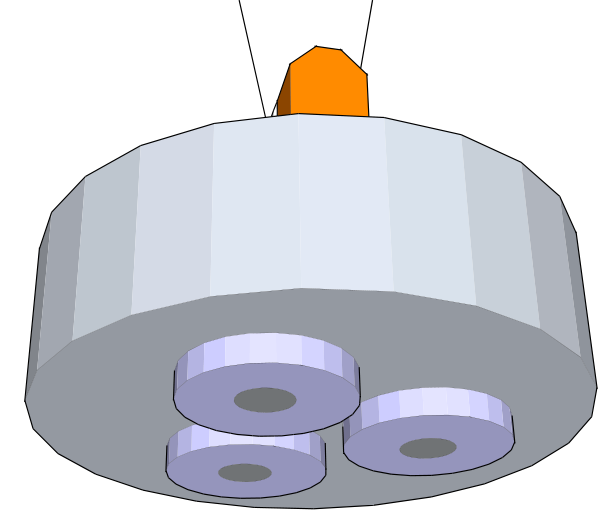
\includegraphics[width=0.3\textwidth]{Billeder/Electromagnet.png}
        \end{subfigure}

% \onslide<2-> \scalebox{0.8}{ \begin{subfigure}{0.98\textwidth}
%         \centering
%         \begin{tikzpicture}
%         \draw [fill = black, ultra thick] (-0.1,0) circle [radius=0.5];;
%         \draw [fill = black, ultra thick] (1.1,0) circle [radius=0.5];;
%         \draw [fill = black, ultra thick] (0.5,1) circle [radius=0.5];;

%         \draw [gray, ultra thick] (0.5,0.35) circle [radius=1.5];;


%         %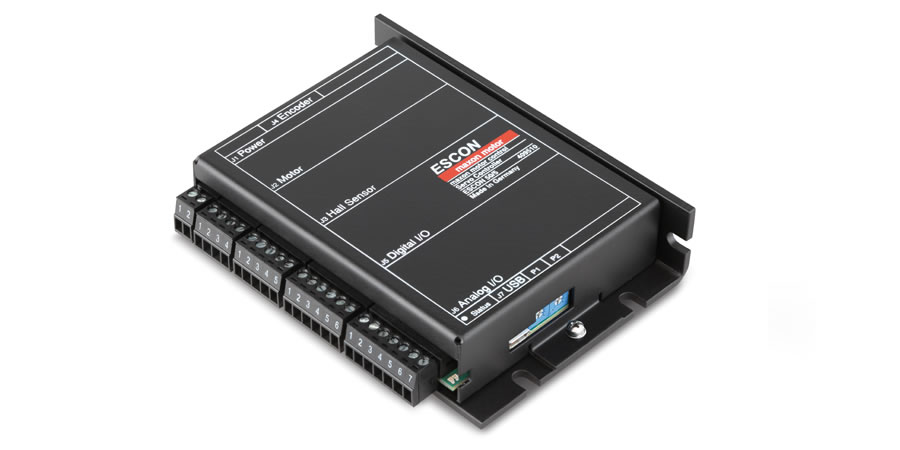
\includegraphics[width=0.5\textwidth]{Billeder/Escon_fig}
%         \end{tikzpicture}
%         \end{subfigure}
%         }

\vspace{0.45cm}
\onslide<3->  \begin{subfigure}{0.98\textwidth}
        \centering
        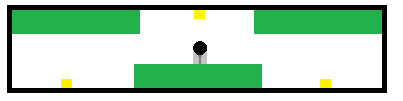
\includegraphics[width=0.5\textwidth]{Billeder/AngleSensor}
        \end{subfigure}     


\end{figure}

\end{column}
\end{columns}

\end{frame}



%%%%%%%%%%%%%%%%%%%%%%%%%%%%%%%%%%%%%%%%%%%%%%%%%%%%%%%%%%%%%%%%%%%%%%%%%%%%%%%%%%%

\begin{frame}{Optimering}{}


  \begin{itemize}
    \item<1-> Statisk friktion
  \end{itemize}

\vspace{0.5cm}
\centering
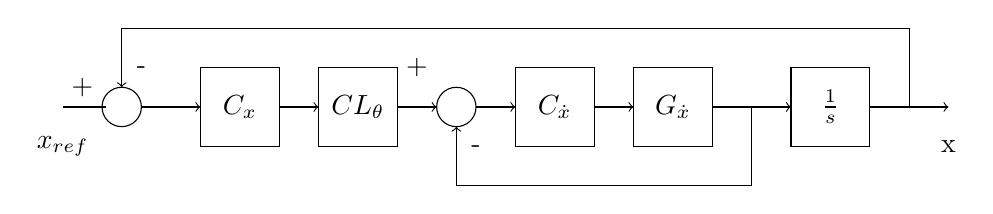
\begin{tikzpicture}

\draw  (-6,1.5) rectangle (-5,0.5);
\draw  (-4.5,1.5) rectangle (-3.5,0.5);
\draw  (-2,1.5) rectangle (-1,0.5);
\draw  (-0.5,1.5) rectangle (0.5,0.5);
\draw  (1.5,1.5) rectangle (2.5,0.5);
\draw  (-2.75,1) ellipse (0.25 and 0.25);
\draw  (-7,1) ellipse (0.25 and 0.25);
\draw (-7.75,1) -- (-7.2,1);

\draw [->](-6.75,1) -- (-6,1);

\draw [->](-5,1) -- (-4.5,1);

\draw [->](-3.5,1) -- (-3,1);

\draw [->](-2.5,1) -- (-2,1);

\draw [->](-1,1) -- (-0.5,1);

\draw [->](0.5,1) -- (1.5,1);

\draw [->](2.5,1) -- (3.5,1);

\draw [->](1,1) -- (1,0) -- (-2.75,0) -- (-2.75,0.75);

\draw [->](3,1) -- (3,2) -- (-7,2) -- (-7,1.25);

\node at (-5.5,1) {$C_x$};
\node at (-4,1) {$CL_\theta$};
\node at (-1.5,1) {$C_{\dot{x}}$};
\node at (0,1) {$G_{\dot{x}}$};
\node at (2,1) {$\frac{1}{s}$};
\node at (-7.5,1.25) {+};
\node at (-6.75,1.5) {-};
\node at (-3.25,1.5) {+};
\node at (-2.5,0.5) {-};
\node at (-7.75,0.5) {$x_{ref}$};
\node at (3.5,0.5) {x};
\end{tikzpicture}
 \end{frame}










%%%%%%%%%%




% \begin{frame}{Optimering}{}


%  \begin{minipage}[H]{0.3\linewidth}
%   \begin{itemize}
%     \item<1-> Static fiction
%   \end{itemize}
%   \end{minipage}

%   \vfill

%   \begin{center}
%   \scalebox{0.8}{
%   \begin{tikzpicture}
%   \draw  (-6,0.25) ellipse (0.25 and 0.25);
% \draw[->,thick] (-7.25,0.25) -- (-6.25,0.25);
% \draw  (-4.75,-0.25) rectangle (-2.75,0.75);
% \draw  (1.25,0.75) rectangle (3.25,-0.25);

% \node at (2.25,0.25) {$G_\dot{x}$};
% \draw  (4.25,0.75) rectangle (5.25,-0.25);
% \node at (4.75,0.25) {$\frac{1}{s}$};
% \draw[->,thick] (7.75,0.25) -- (7.75,1.75) -- (-6,1.75) -- (-6,0.5);
% \node at (6.5,0.25) {x};
% \draw[->,thick] (5.25,0.25) -- (6.25,0.25);

% %\draw  (7.25,0.75) rectangle (9.25,-0.25);

% \draw[->,thick] (-5.75,0.25) -- (-4.75,0.25);
% \draw[->,thick] (3.25,0.25) -- (4.25,0.25);



% \node at (-6.5,0.5) {+};
% \node at (-5.75,0.75) {-};
% \node at (-7.75,0.25) {x};

% \node at (-3.75,0.25) {$C_x$};

% \draw  (-1.75,-0.25) rectangle (0.25,0.75);
% \node at (-0.75,0.25) {$CL_\theta$};
% \draw[->,thick] (-2.75,0.25) -- (-1.75,0.25);
% \draw[->,thick] (0.25,0.25) -- (1.25,0.25);

% \end{tikzpicture}}
% \end{center}
%   \end{frame}




%%%%%%%%%%%%%%%%%%%%%%%%%%%%%%%%%%%%%%%%%%%%%%%%%%%%%%%%%%%%%%%%%%%%%%%%
\section{Konklusion}




\begin{frame}{Konklusion}{}
  \begin{itemize}
    \item<1-> Analyse af kran  
    \item<2-> Modeller er blevet udledt på baggrund af analyse  
    \item<3-> Parameter estimeringer 
    \item<4-> Root locus er benyttet under udvikling af regulatorer 
    \item<5-> Strøm offset kan kompensere for statisk friktion
    \item<6-> Kaskade kobling  
  \end{itemize}
\end{frame}




\begin{frame}{Demonstration}{Simon}
  \begin{itemize}
    \item<1-> Kontrol lab
  \end{itemize}
\end{frame}
%%%%%%%%%%%%%%%%